% -*- Mode:TeX -*-
% LaTeX template for CinC papers                   v 1.1a 22 August 2010
%
% To use this template successfully, you must have downloaded and unpacked:
%       http://www.cinc.org/authors_kit/papers/latex.tar.gz
% or the same package in zip format:
%       http://www.cinc.org/authors_kit/papers/latex.zip
% See the README included in this package for instructions.
%
% If you have questions, comments or suggestions about this file, please
% send me a note!  George Moody (george@mit.edu)
%
\documentclass[twocolumn]{cinc}
\usepackage{graphicx}
\usepackage{dblfloatfix}
\usepackage{url}
\begin{document}
\bibliographystyle{cinc}

% Keep the title short enough to fit on a single line if possible.
% Don't end it with a full stop (period).  Don't use ALL CAPS.
\title{Quantum Semiprime Factorization: Leveraging Grover's Algorithm for Efficient Prime Decomposition}

% Both authors and affiliations go in the \author{ ... } block.
% List initials and surnames of authors, no full stops (periods),
%  titles, or degrees.
% Don't use ALL CAPS, and don't use ``and'' before the name of the
%  last author.
% Leave an empty line between authors and affiliations.
% List affiliations, city, [state or province,] country only
%  (no street addresses or postcodes).
% If there are multiple affiliations, use superscript numerals to associate
%  each author with his or her affiliations, as in the example below.

% \author {Jacob Collins$^{1}$, Jaime Raigoza$^{1}$, Sam Siewert$^{1}$ \\
\author{Jacob Collins$^{1}$, Jaime Raigoza$^{1}$, Sam Siewert$^{1}$ \\
\ \\ % leave an empty line between authors and affiliation
 $^1$ California State University, Chico, United States}

\maketitle

% LaTeX inserts the ``Abstract'' heading in the proper style and
% sets the text of the abstract in italics as required.
\begin{abstract}

  This paper details some of the first steps that our research group has
  taken towards a practical demonstration of quantum advantage. 

  Grover's search algorithm can be leveraged to efficiently compute the inverse 
  of many functions; this is addressed both from a general perspective, as well as
  specific applications, including inversion of multiplication,
  thereby finding the factors of semiprimes with greater efficiency 
  than classical HPC methods and similar existing quantum algorithms.
  
  RSA encryption relies on the fact that the multiplication of large
  prime numbers is a trap-door function- computationally trivial to compute
  the semiprime product, but classical methods of finding prime components
  is so computationally expensive that it can be considered nearly impossible
  at a large scale. This principle is the backbone of 
  modern-day cybersecurity~\cite{FergusonSchneier2003}.

  % In quantum computing, SP (semiprime) factoring is typically performed 
  % with Shor's algorithm, but it is possible to achieve the same results
  % more efficientily via Grover's algorithm\cite{quantum_factoring, grover}. 
  %
  \textbf{Key terms:} Semiprime, superposition, entanglement, Grover's algorithm, 
  Shor's algorithm, quantum fourier transform, adjoint, RSA encryption, 
  quantum advantage, RSA number, reversible function, trap-door function,
  quantum circuit, scaling, parallel, CUDA, CUDA-Q, sieve, time complexity.
  %
  % The abstract with its heading should not be more than 100 mm long,
  % which is equivalent to 25 lines of text. Leave 2 line spaces at the
  % bottom of the abstract before continuing with the next heading.


\end{abstract}
% LaTeX inserts the extra space here automatically.

\section{Introduction}

The practicality of applied quantum computing is a topic of much debate,
and there are not yet many examples of quantum computers being able to out-perform
their classical counterpart, a feat known as quantum advantage.

Quantum algorithms have been in development at a theoretical level for
decades, but the application of these methods is still in early stages.
It is quite common to find code which implements a quantum algorithm like
Grover's\cite{grover} or Shor's\cite{shor}, but very often these 
programs are hard-coded, and only
work for a small handful of specific values\cite{shors_ibm}.

This paper describes the generalized use of Grover's algorithm as the
inverse of some function $F(x, y) = z$, with demonstrated applications
inverting the arithmetic functions addition and multiplication. Specifically,
our implementation can generate and simulate a circuit to find the distinct prime
factors of any given semiprime.

\begin{figure}[ht]\label{fig:FIGURA1}
\centering
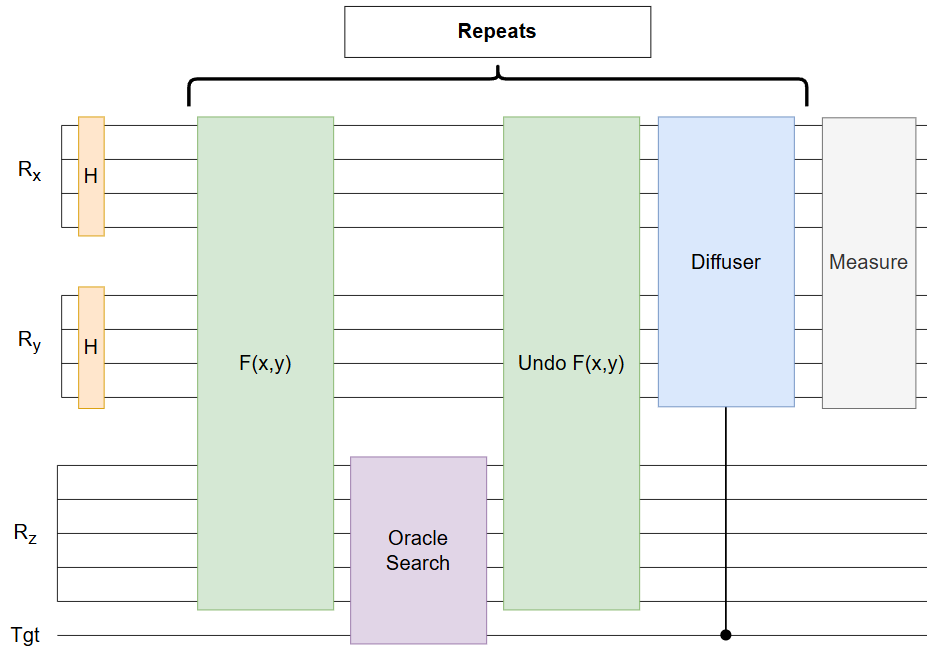
\includegraphics[width=7.9cm]{grover_inversion.png}
% 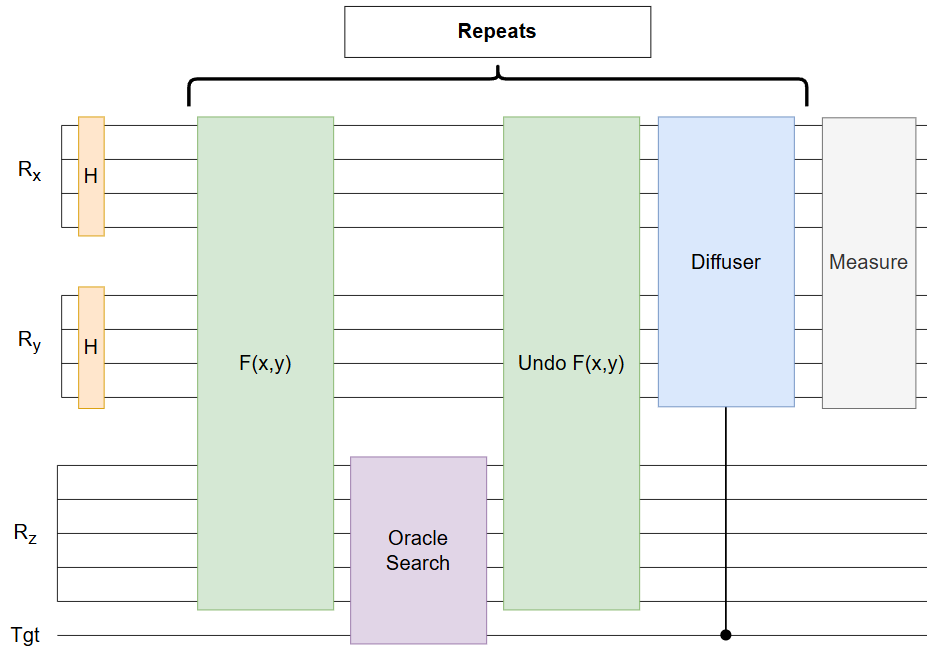
\includegraphics[width=15.8cm]{grover_inversion.png}
% 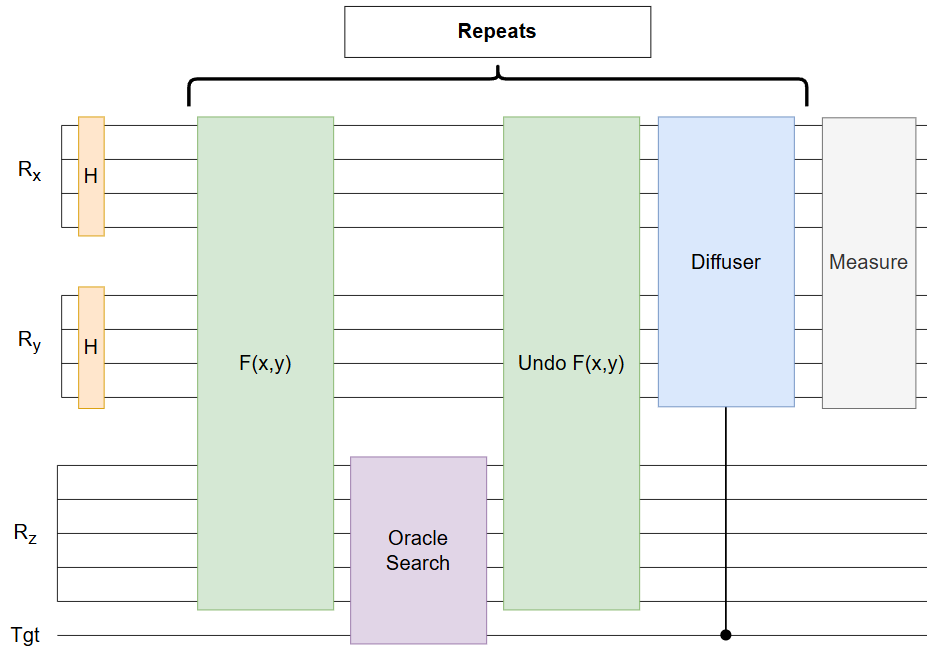
\includegraphics[width=14cm]{grover_inversion.png}
\caption{General circuit diagram for Grover's Algorithm, used to find 
the inputs $x, y$ for which $f(x,y)=z$, for some known output $z$.}
\end{figure}

  \subsection{Goals}

  The objective of this research is to clearly demonstrate quantum advantage 
  by showing clear speed-up to solve the same problem at the same scale.

  % Some of the major limitations for applied quantum computing are 
  % the number of qubits required to perform a given task, the likelihood of errors
  % in measurement, and the overhead associated with running circuits on real-world
  % quantum computers. 
  
  % Today many functions are reversible with digital computing (while not adiabatic), 
  % but not all. For example, a discrete cosine transformation or Fourier transform 
  % can be reversed, but for other algorithms, the only option for reversal is 
  % brute-force search or getting lucky. For example, optimizing a function can be 
  % done by trial and error with Monte Carlo guessing, and the possible solutions can 
  % be quickly tested for optimality, but many functions cannot be easily optimized 
  % short of brute-force search or Monte Carlo. Other examples being considered by 
  % our group include subset sums, path planning, and machine learning gradient descent.
  %
  While the semiprime factoring problem is just one algorithm where quantum circuits 
  should have significant advantage over parallel factoring, 
  the goal of this research is to concretely show that this particular problem is 
  in fact a clear case of quantum advantage.

  One of the major intentions for this paper is demonstration of the broad utility of Grover's 
  algorithm.%, and to provide a general reference
  %for how Grover's algorithm may be used to invert a given function.

  Furthermore, the longer-term goal is to identify the types of algorithms that 
  likewise may have significant quantum advantage based upon reversible functions.
  % Grover's algorithm can be used to provide a very efficient search, 
  % which is in essence a content addressable memory that works at a scale limited only by qubit scaling.

  \subsection{Motivation}

  Semiprime factoring is an ideal problem for demonstrating quantum advantage,
  as it is both challenging to compute classicaly, and has wide-reaching
  impact if efficient solutions are found.

  Semiprime factoring is known to have a high time complexity due to the nature of
  prime number generation with a sieve (filters out all non-primes) and trial division search.
  This problem in particular becomes complex for large size semiprimes commonly used in 
  encryption, which might be 4096 bits or more. 
  Even a 128-bit semiprime, which is the product of two 64-bit primes requires time complexity
  that is beyond polynomial, and therefore requires a parallel computer to solve today. 

  This is important since the simplicity of multiplying two large primes enables fast encryption of data, 
  but the complexity of factoring semiprimes ensures privacy so that data can only be accessed by someone possessing a private key 
  (one of the primes that compose the semiprime used for encryption).

  Data privacy hinges on this one-way function, called a trap-door, where factoring 
  is beyond P complexity, but trivial if one possesses the required key. 

  % If a quantum computer makes SP factoring as simple as SP computation, given a 
  % reversible quantum circuit, then this means all encryption can potentially 
  % be broken by such a quantum circuit. 
  
  The only safety now for encryption is scaling the key size (semiprime) to keep 
  it larger than the largest quantum computer number of qubits.

  For example, the RSA number 250, which is 892-bits long, was only recently 
  factored using a parallel computer with the best known SP factoring 
  method known right now~\cite{Bai2016}.

  The idea of factoring 4096 or bigger is nearly impossible even with the largest parallel computers available~\cite{FergusonSchneier2003}. 

  However, a quantum computer has a much lower time complexity if the number of qubits
  can be scaled to implement a quantum circuit that can factor a semiprime. Ongoing research
  at China State Key Laboratories suggests that they have been making significant
  progress in breaking RSA encryption, considering their 48-bit demo using 10 qubits
  in 2022~\cite{yan2022factoringintegerssublinearresources}. 
  
  Furthermore, they claim
  that with the techniques they have been using, it would be possible to break
  RSA 2048 with a quantum circuit which needs only 372 qubits, far less than the
  1,121 qubit machine currently available in the United 
  States with IBM's Condor~\cite{abughanem2024ibmquantumcomputersevolution}.

  % The typical approach to semiprime factoring on a quantum computer is 
  % with Shor's algorithm, but there are many drawbacks to this approach,
  % and has not yet been observed to be practically advantageous.

  If it can be verified that SP factoring with Grover's algorithm
  uses significantly less qubits than Shor's, has less error, or has less overhead,
  then the application of quantum semiprime factoring at a meaningful scale 
  will be feasible far sooner.

\section{Literature Review}

  \subsection{Grover's Algorithm}

  Grover's Algorithm is a quantum computing method 
  that can be used to search a database of $N$ values in $O(\sqrt{N})$ time 
  rather than the naive classical time complexity of $O(N)$\cite{grover}. 

  The exact number of iterations required varies on a case-by-case basis,
  but is typically expressed as follows: in a search for one matching input
  state, $\frac{\pi}{4}\sqrt{N}$ iterations are required, and in a search
  for $k$ valid input states, $\sqrt{\pi}{4}\cdot \sqrt{\frac{N}{k}}$
  iterations are required, where $N$ is the size of the search domain.

  In most cases, $N=2^n$, where $n$ is the number of bits needed to represent
  the target value. This is by no means a steadfast rule, and is meant as 
  a helpful starting point for any confused readers attempting to implement
  something similar themselves.
  
  Given a function $f(x)=y$, where $x$ is unknown (index, prime factors, 
  sum components, etc.), and $y$ is known (array value, semiprime/product, 
  sum, etc.), Grover's algorithm effectively takes the role of $f'(y)=x$, 
  allowing for a potential speedup in finding whatever input (s) to $f(x)$
  will return $y$, provided that it is much faster to compute $f(x)$ than
  whatever classical methods might be used to otherwise solve for $x$ given $y$.

  This speedup comes from the fact that Grover's algorithm requires 
  $O(\sqrt{y})$ iterations, each of which have a time complexity proportional
  to that of $f(x)$.

  \subsection{Shor's Algorithm}

  Shor's algorithm is the most well-known approach to prime factorization
  in quantum computing. However, there are many drawbacks to this approach,
  the most notable of which being the need to take measurements mid-circuit
  and essentially re-run with new values afterwards, which introduces a 
  significant amount of overhead. Even recently improved versions of Shor's
  algorithm still require a minimum of $2n+1$ qubits, and tend to be 
  extremely sensitive to noise, which leads to high error\cite{quantum_factoring,shor}.

  Furthermore, when it comes to more concrete applications of Shor's algorithm,
  a full-scale implementation of this algorithm to factor an $n$-bit number
  may require up to $5n+1$ qubits for accurate results, and require 
  on the order of $n^3$ operations~\cite{quantum_fac_efficient}.

  \subsection{Quantum Factoring Algorithm with Grover Search}

  S. Whitlock et al.\ present a method of SP factoring with Grover's
  algorithm. The implementation in their paper is highly optimized,
  and modifies the target value in their circuit from some semiprime $N$,
  to $M$, a reduced number uniquely tied to $N$, which has unique factors 
  $p$ and $q$ which can be used to calculate $a, b$, the prime factors of 
  $N$~\cite{quantum_factoring}. 
  
  This optimization from $N$ to $M$ allows the implementation to ignore
  the trivial prime factors $2$ and $3$, and requires fewer qubits than would
  otherwise be needed to search for prime factors of $N$.

  While this approach is admirable, it introduces a level of complexity 
  that may hinder a learner's understanding of the mechanics at work,
  so the implementation shown in section\ \ref{sec:Methodology} forgoes
  this abstraction from $N$ to $M$, and instead implements an oracle which
  searches directly for prime factors $a$ and $b$ of a semiprime $N$.

\section{Methodology}\label{sec:Methodology}

Quantum algorithms take advantage of superposition and entanglement,
which enables many methods of computation which are otherwise impossible
with a classical computer. For example, by placing a set of $n$ qubits 
(otherwise known as a qubit \textbf{register}) in superposition, that register
simultaneously represents every value which can be represented in $n$ bits,
until measured. Once measured, a register in uniform superposition will 
collapse into one of these states with equal likelihood.

% In a given register $R_n$ with $n$ qubits, values are represented in binary,
% such, for example, if some number $N=3$ were to be represented classically
% with $n=4$ bits, it might be seen in binary as $0011$, and on a qubit
% register that number may be represented similarly as $| 0011 \rangle$.
%
  \subsection{The Use of Grover's Algorithm for General Function Inversion} 

  % Operations can be performed on a set of input registers that start in uniform 
  % superposition, and these operations will affect each potential state individually. 
  % The properties of superposition are utilized by Grover's Oracle to selectively 
  % modify the states $|x,y\rangle$ in the input registers $R_x$ and $R_y$,
  % marking them as valid by setting them to $-|x,y\rangle$, only when the output register
  % $R_z$ matches some known search term $z$. An outline of a quantum circuit for
  % Grover's algorithm is seen in Figure~\ref{fig:FIGURA1}.
  
  This use of Grover's algorithm involves three main parts: some function with
  one or multiple inputs, the oracle which filters for states in which the
  desired output was observed, and the diffuser, which increases the probability 
  of observing inputs from the correct state. An overview of this circuit is
  shown in Figure~\ref{fig:FIGURA1}.

  The oracle in Grover's algorithm performs a controlled operation which is meant
  to differentiate states $-|x,y\rangle$ that do result in the wanted target $z$ from 
  states $|x,y\rangle$ that do not result in the target $|z\rangle$.
  
  \begin{figure}[!ht]
  \centering
  % 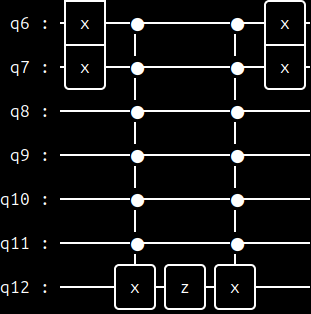
\includegraphics[width=6.0cm]{oracle_15.png}
  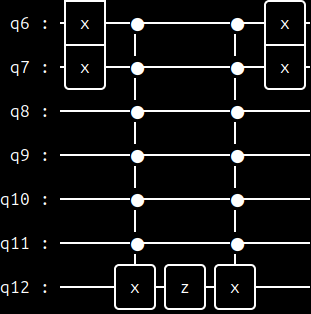
\includegraphics[width=5.0cm]{oracle_15.png}
  % 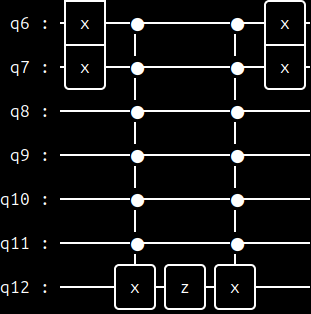
\includegraphics[width=7.9cm]{oracle_15.png}
  \caption{Example circuit diagram for Grover's oracle marking entangled states 
  of the output register ($R_z=[q_0,q_{11}]$) via the target qubit ($q_{12}$), where
  $R_z=|15\rangle$.}\label{fig:FIGURA2}
  \end{figure}

  \begin{figure}[!h]
  \centering
  % 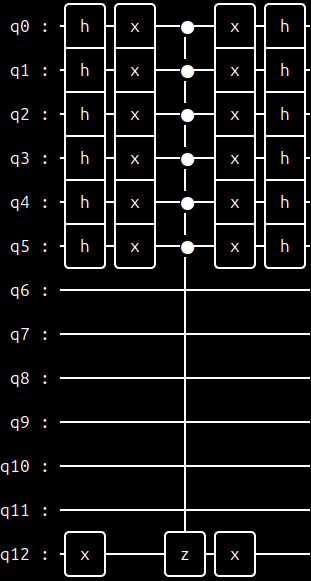
\includegraphics[width=7.9cm]{diffuse.png}
  % 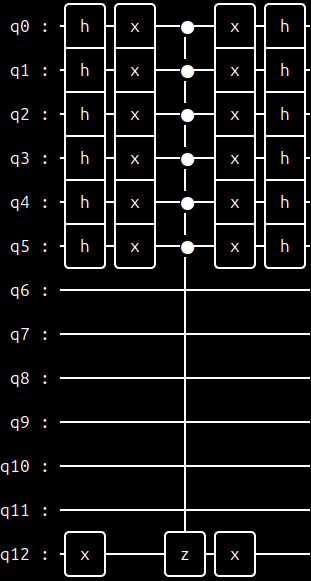
\includegraphics[width=5.0cm]{diffuse.png}
  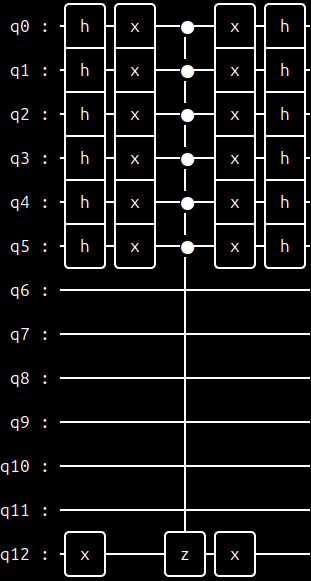
\includegraphics[width=4.2cm]{diffuse.png}
  \caption{Example circuit diagram for a diffuser which amplifies the probability that
  measurement will result in a state which has been marked by the oracle.
  Input registers $R_x$ and $R_y$ ($[q_0,q_2]$ and $[q_3,q_5]$) are now 
  more likely to be measured in a state such that $f(R_x,R_y)$ results in $R_z=|z\rangle$.}\label{fig:FIGURA3}
  \end{figure}

  Figure~\ref{fig:FIGURA2} shows an example of the oracle searching for the state $z=15$,
  or rather, $R_z=|001111\rangle$. To implement a circuit which can selectively target
  $z=15$, Toffoli gates (controlled-NOT) are applied on $R_z[0]$ and $R_z[1]$, 
  so that states where $R_z=|001111\rangle$ will temporarily be in
  state $R_z=|111111\rangle$, and the multi-controlled Toffoli gates\cite{multi_toffoli}
  will apply only for the desired states. These operations are then performed again,
  returning all but the target qubit (which has the Z-gate applied) to their original
  states.

  The diffuser in Grover's algorithm (Figure~\ref{fig:FIGURA3}) can then increase the 
  probability of observing $-|x,y\rangle$ (states which have been marked by the oracle) 
  through a process known as inversion about the mean.

  \subsection{Semiclassical Arithmetic} 

  As a proof of concept (prior to the release of~\cite{quantum_factoring}),
  a function $f(x,y)=x+y$ is defined such that $R_x=|x\rangle$, $R_y=|y\rangle$,
  and after performing $f(R_x,R_y)$, the output register $R_z$ shall be in the
  state $|x+y\rangle$.
  
  This approach was implemented in a similar manner to a classical full-adder,
  and has been observed to work in simulation with perfect accuracy~\cite{quantum_full_adder}.

  The semiclassical full-adder indeed works with Grover's algorithm. Input states were
  filtered to only measure inputs which resulted in a sum matching some given value.
  This is a trivial problem however, and only has potential usefulness due to the 
  relationship between multiplication and addition.

  Unfortunately, semiclassical multiplication requires direct measurement of $R_x$
  or $R_y$, which would collapse the superposition, so a different approach was
  needed.

  % Semiclassical arithmetic does have significant drawbacks, however. Despite
  % being relatively simple to implement due to the similarity with principles
  % that have a much broader range of documentation, the classical nature of this
  % implementation meant that in order to move to multiplication from this point,
  % the value of one register would need to be measured, and $R_x$ would then be
  % added to $R_z$ a number of times dependent on the value of $y$.
  %
  % Measuring the state of either input register would collapse the superposition,
  % and break the underlying principles on which Grover's algorithm depends. Thus,
  % a different approach became necessary- one that could bridge the gap between 
  % addition and multiplication without needing to measure either register,
  % so that the operation can still work with inputs that are in superposition,
  % allowing the use of Grover's algorithm.

  \subsection{Arithmetic in the Quantum Fourier Domain}\label{sec:qft_arithmetic} 

  The quantum fourier transform, QFT, is a very useful
  operation, typically used to transform a qubit register from the
  computational basis (binary) to the fourier basis (phase).  The QFT operation 
  is defined in great detail by Perez et al.~\cite{quantum_arithmetic}. 
  
  To summarize, given a qubit register $R_x=|x\rangle$
  with $n$ qubits in the computational basis, there are $d=2^n$ potential states $|k\rangle$
  in $|x\rangle$ = $\{|0\rangle, |1\rangle, \ldots, |d-1\rangle\}$, the QFT operation in this
  basis would be defined as:

  \begin{equation}\label{eqn:QFT}
    QFT|x\rangle = \frac{1}{\sqrt{d}} \sum_{k=0}^{d-1}e^{i{\frac{2\pi x k}{d}}}|k\rangle
  \end{equation}

  *It is worth noting that in some cases, a QFT on some $R_x$ may require a series of SWAP
  operations $\{ SWP(q_0,q_{n-1}), SWP(q_1,q_{n-2}), \ldots, SWP(q_{\frac{n}{2}-1},q_{\frac{n}{2}})\}$
  in order for future arithmetic to work as expected.

  Once in the fourier basis, a specific number $x$ may be encoded by applying some
  rotation $\omega_k$ to qubits $q_k \in R_x | q_k=R_x[k]$. The rotation $\omega_k$ applied
  to each qubit $q_k$ can be defined as $\omega_k = \omega^{x k} = e^{i \frac{2\pi x k}{d}}$.

  % The inverse QFT operation, IQFT, is simply the adjoint of QFT, and most 
  % implementations allow you to automatically generate the adjoint of a given operation.
  The inverse QFT operation, IQFT is used to return a qubit register $R_x$ from the fourier basis to the 
  computational basis, retaining the values which have been mapped and operations
  which have been applied to $R_x$.

  Addition of two qubit registers $R_a$ in state $|a\rangle$ and $R_b$ in state 
  $\phi(b)\rangle$ in the fourier basis 
  ($\phi ADD(|a\rangle, |b\rangle)=|a + b\rangle$) may be performed by applying
  controlled rotation gates $R_k$ which rotate qubits $b_j \in R_b$ by 
  $\omega_j=e^\frac{2\pi i}{2^j}$ about the $z$-axis for each 
  qubit $a_l | l \ge k, j=1+l-k$~\cite{quantum_arithmetic}. 

  Multiplication in the quantum fourier domain can be done similarly. In terms of
  a quantum circuit generation implementation, simply treat the previously defined
  addition method as a function which adds the value of one register to another,
  and add some constant multiple $C$ as a parameter, adjusting $\omega_j$ to 
  $\omega_{j,C}=e^{C\cdot \frac{2\pi i}{2^j}}$. Now, to send the product of the two values in $R_x$
  and $R_y$ to $R_z$, do as follows: Add $|R_y|$ controlled $\phi ADD(R, q_c, C)$ gates to each
  $q_x$ in $R_x$, which will add the value of $|C\cdot x\rangle$ to $R_z$ where $C=2^u$ for
  each $q_u \in R_y \iff q_y = |1\rangle$. This is, in essence, performing repeated scaled addition from $R_x$ onto
  $R_z$, but the scaling factor is the powers of two corresponding to qubits in $R_y$, which
  in tandem is cumulatively equivalent to adding $|x\cdot y\rangle$ to $R_z$~\cite{quantum_arithmetic}.

  \subsection{Semiprime Factoring with Grover's Algorithm}

  After implementing the QFT arithmetic methods and the oracle and diffuser for
  grover's, it is trivial to implement a SP factoring circuit. Our implementation
  follows the diagram in Figure~\ref{fig:FIGURA1}, while substituting $F(x,y)$ for
  the $\phi MULT(R_x, R_y)$ operation described at the end of section 
  \ \ref{sec:qft_arithmetic}.

  The only fine-tuning necessary here was to add additional bits to the $R_z$ register.
  Typically, only $\lceil \log_2(N)\rceil$ qubits are needed to represent some number $N$,
  and while that is true, we experienced something that might be considered quantum integer
  overflow before increasing the number of qubits in $R_z$. Prime factors $a,b$ of $N$ may be as
  little as one bit smaller than $N$, and due to the fact that $R_x$ and $R_y$ representing $a,b$
  are in superposition, that meant that all numbers up to $2^{n-1}$ were being included
  in the superposition for both $a$ and $b$, resulting in products far larger than could
  be represented in $R_z$, which in turn led to false positives due to products that were
  some sum of powers of 2 greater than $n$.

  The temporary solution we found was to simply decrease the size of $R_x$ and $R_y$ to 
  $\lceil \log_2(\frac{N}{3})\rceil$, and set the size of $R_z$ to double that, to ensure no
  further overflow could occur.

  % \subsection{Quantum Circuit Simulation}

  % It can be very expensive and time-consuming to run quantum circuits on real-world
  % quantum computers, especially for problems which require a large number of qubits.
  % Simulation is a strong solution to this issue; the math involved with qubits
  % is known, so the state of a quantum circuit can be tracked properly throughout 
  % execution.

  % The methods described in this paper have been programmed using CUDA-Q in C++. This
  % method of simulation allows for generalized circuit generation algorithms, and
  % the ability to verify that a solution theoretically works at larger problem scales
  % than would be possible to attempt on an actual quantum computer given the current 
  % limitations of the quantum computing industry.

\section{Results and Discussion}

To date, we have preliminary results based on CUDA-Q simulation of quantum circuits, 
which have been compared to classic parallel methods to generate primes with a sieve 
and search them for modulo zero factoring. 

This work is still in progress, but we have a working implementation of Grover's 
algorithm with the CUDA-Q simulation which can estimate the time to factor any 
semiprime up to the current scaling limits of the CUDA-Q simulation\cite{quantumfactoring_github}. 

We first plan to compare the Grover quantum circuit to our best parallel sieve 
and modulo search with this scale-out with SDSC Expanse.

  \subsection{Accuracy and Limitations}

  On our CSU Chico A100 system, 
  we have been able to scale this implementation up to a total of 32 qubits,
  used to find the prime factors $47\times13=611$, where $611$ is a 10-bit semiprime. This
  performance is due to the sub-optimality of the current implementation, as we have
  not yet introduced the search-term reduction from $N$ to $M$ as is done by S. Whitlock 
  et al.\cite{quantum_factoring}. 

  Due to the exploratory nature of this work, the initially sub-optimal nature of our 
  implementation is intentional, because it allows for a more direct view of the inputs
  and outputs in our circuit.

  For context, our current implementation uses $4 \lceil \log_2(\frac{N}{3})\rceil$ qubits
  to find the prime factors of an $n$-bit semiprime, whereas the design by S. Whitlock 
  et al.\cite{quantum_factoring} uses up to $2n-5$ qubits, which allowed them to simulate circuits which found
  prime factors of up to $35$-bit semiprimes, using up to a total of $65$ qubits. 
  The limiting factor for our simulations is VRAM, so it is expected that after implementing 
  the optimizations from S. Whitlock et al.,\ our simulations should be able to scale up to 
  $18$-bit semiprimes on the current equipment.

  % In simulation, our implementation of quantum semiprime factoring with Grover's algorithm
  % has $100\%$ accuracy on all observed simulation runs with 100 shots each. The expected
  % accuracy is very near $100\%$, and simulating with a greater number of shots might allow us
  % to see a handful of the expected erronious results, but the simulations are rather time 
  % consuming (finding prime factors of 611 took over 20 minutes on the current machine), 
  % and the current priority is verification of a working circuit, which has indeed been observed.
  %
\section{Conclusion}

\balance

Grover's algorithm has been demonstrated to be a highly versatile function,
able to invert almost any function that can be implemented on a quantum 
computer with inputs in superposition.

Quantum methods of SP factoring have been developing at a quick pace,
and it will most likely not be very long before practical examples
of quantum advantage may be seen.

\section{Future Work}
 
The current priority regarding the quantum circuit is to implement the optimizations
mentioned by S. Whitlock et al.\ to substitute the search term $N$ with the smaller
search term $M$, which should reduce the number of qubits needed from 
$4 \lceil \log_2(\frac{N}{3})\rceil$ to $2n-5$.

We have recently gained access to resources at the San Diego Supercomputing 
Center (SDSC) Expanse cluster via an NSF allocation grant. This equipment will allow us to
simulate on far larger problem scales, and by tracking the number of operations (quantum gates)
used at different problem scales and comparing those counts against the number of operations
performed in our classical parallel solution, we should be able to simulate circuits at a scale
much larger than our current limitation of $\approx 32$ qubits.

\section*{Acknowledgments}  
% This section is not numbered.
% 
Jacob Collins has been funded by Chico State Enterprises as an undergraduate research assistant
through funding provided by the Department of Energy via a grant titled: \emph{QIST in the CSU:\ 
Expanding Access to Quantum Information Science and Technology.}

% LateX generates the ``References'' heading automatically and switches
% to 9 point type for the bibliography.  Please  use BibTeX and
% follow the examples in the sample 'refs.bib' file to enter your references.
\bibliography{refs}

% If you don't use BibTeX (why not?) , comment out or remove the previous
% line, and uncomment the following lines up to the ``}\end{bibliography}''
% line below:
%\begin{thebibliography}{99}{ %\small
% \bibitem{tag} (General form) J. K. Author, ``Name of paper,''
%   \emph{Abbrev. Title of
%   Periodical}, vol. x, no. x, pp. xxx--xxx, Abbrev. Month, year. 

% \bibitem{ito}  M. Ito et al., ``Application of amorphous oxide TFT to
%   electrophoretic display,'' \emph{J. Non-Cryst. Solids}, vol. 354, no. 19,
%   pp. 2777--2782, Feb. 2008.
  
% \bibitem{fardel}  R. Fardel, M. Nagel, F. Nuesch, T. Lippert, and
%   A. Wokaun, ``Fabrication of organic light emitting diode pixels by
%   laser-assisted forward transfer,'' \emph{Appl. Phys. Lett.}, vol. 91,
%   no. 6, Aug. 2007, Art. no. 061103.
  
% \bibitem{buncombe} J. U. Buncombe, ``Infrared navigation Part I: Theory,''
%     \emph{IEEE Trans. Aerosp. Electron. Syst.}, vol. AES-4, no. 3,
%     pp. 352--377, Sep. 1944.
      
% Uncomment the following line if you are not using BibTeX.
%}\end{thebibliography}


% LaTeX inserts the ``Address for correspondence'' heading.
\begin{correspondence}
Jacob Collins\\
1565 Filbert Avenue, Chico, CA 95926\\
jbcollins@csuchico.edu
\end{correspondence}

\end{document}

